\documentclass[11pt,xcolor=svgnames]{beamer}
\usepackage{dsfont,natbib,setspace,changepage,multirow,dsfont}
\mode<presentation>

% replaces beamer foot with simple page number
\setbeamertemplate{navigation symbols}{}
%\setbeamerfont{frametitle}{series=\bfseries}
\setbeamercolor{frametitle}{fg=Black}

\setbeamertemplate{footline}{
   \raisebox{5pt}{\makebox[\paperwidth]{\hfill\makebox[20pt]{\color{gray}\scriptsize\insertframenumber}}}}

% colors
\newcommand{\theme}{\color{Maroon}}
\newcommand{\bk}{\color{black}}
\newcommand{\nv}{\color{Navy}}
\setbeamercolor{itemize item}{fg=gray}

\begin{document}

\setcounter{page}{0}
\begin{frame}[plain]
\begin{center}


{\bf \Large Measuring Segregation in High Dimensions}


\vskip 1cm
Matthew Gentzkow, Chicago Booth and NBER\\
Jesse M. Shapiro, Brown and NBER\\
Matt Taddy, Chicago Booth


\end{center}
\end{frame} 

\begin{frame}


There's a big lit on measuring change in polarization/segregation.

\vskip .5cm
For example:
\begin{itemize} 
\item The $d$-vector  $\mathbf{c}_{tr} = [c_{tr1} \ldots c_{trd}]$ counts the number of members of race $r$ in each neighborhood
$j$ at time $t$.\\
{\color{black!50}
Or, compare across cities/countries/school districts/etc.}
\item 
Segregation measure maps counts $\left\{ \mathbf{c}_{tr}\right\} _{r=1}^{R}$
into scalar $s_{t}$
\item Use $s_1 \dots s_T$ to answer questions like
\item[]~~~~{\theme ``Has this city become more segregated over
time?''}
\end{itemize}

\vskip .5cm
Today's talk is about how to build $s_t$  when $d$ is really big.

\end{frame}


\begin{frame}

Current indices are derived from sets of stated desirable properties.


\vskip .5cm
Example: Atkinson index (Frankel and Volij 2010)
\[
s_{t} = 1 - \sum_{j} \sqrt{\frac{c_{t0j}}{m_{t0}}~
\frac{c_{t1j}}{m_{t1}}}
\]
for two groups (e.g., races) $r=0$ and $r=1$, where $m_{tr} = \sum_j c_{trj}$.

\vskip .5cm
This builds on an earlier literature that provides isolation, dissimilarity, mutual information, gini, and other indices.

\end{frame}


\begin{frame}

Are we after properties of the sample or of the DGP?

\vskip .2cm
That is, if the data are consistent with race-blind assignment do we
want to say that segregation is low?

\vskip .2cm
{\color{black!50} e.g., Cortese et al. (1976), Carrington and Troske (1997) both do.}

\vskip .5cm
Think of Atkinson as 
\[
\hat s_{t} = 1 - \sum_{j} \sqrt{\hat p_{t0j}~
\hat p_{t1j}}
\]
where $\mathbf{p}_{trj}$ is the true probability that a member of $r$ lives in $j$ at $t$. 


\vskip .5cm
This distinction is unimportant if $\hat s_t \approx s_t$.

\vskip .2cm
It is so for residential segregation because  zipcodes are large.

\vskip .2cm
But estimation bias becomes very important as units get smaller...

\end{frame}

\begin{frame}{Number of Districts Small}

1 million students

\begin{center}\vskip -1cm
\includegraphics[width=0.45\textwidth]{../graphs/montecarlo/zipf_shorttail}
\end{center}
\vskip -2cm
\hfill 100 districts.

\end{frame}

\begin{frame}{Number of Districts Medium}

1 million students

\begin{center}\vskip -1cm
\includegraphics[width=0.45\textwidth]{../graphs/montecarlo/zipf_mediumtail}
\end{center}
\vskip -2cm
\hfill 1000 districts

\end{frame}

\begin{frame}{Number of Districts Large}

1 million students

\begin{center}\vskip -1cm
\includegraphics[width=0.45\textwidth]{../graphs/montecarlo/zipf_longtail}
\end{center}
\vskip -2cm
\hfill 10,000 districts

\end{frame}

\begin{frame}{Number of Districts Very Large}

1 million students

\begin{center}\vskip -1cm
\includegraphics[width=0.45\textwidth]{../graphs/montecarlo/zipf_verylongtail}
\end{center}
\vskip -2cm
\hfill 100,000 districts

\end{frame}


% \begin{frame}{Different Ordering}

% \begin{center}
% \includegraphics[width=0.5\textwidth]{../graphs/montecarlo/districts}
% \end{center}

% \end{frame}

\begin{frame}{This paper}


We build a utility-based model of assignment to groups, \\then define a segregation measure within this model.

\vskip .5cm
$\Rightarrow$ a Big-response-dimension multinomial logistic regression.  

\begin{itemize}
\item Use penalization to control finite-sample behavior
\item Implement distributed estimation for scalability
\end{itemize}
{\color{black!50} We control for 100s of covariates and 1000s of random effects.}

\vskip .5cm
Applications to polarization/segregation in
\begin{itemize}
\item congressional text (gop vs. dem, south vs. north)
\item internet browsing (white vs. black)
\item grocery store purchases (college educated vs. not)
\end{itemize}

\end{frame}

\begin{frame}

{\theme Multinomial logit model:}
Each individual $i$ in period $t$ \\makes $m_{it}$ choices over units
$j$ to maximize utility
\[
\eta_{itj} + \varepsilon_{itj} = \alpha_{jt}+\mathbf{u}_{it}'\boldsymbol{\gamma}_{jt}+\varphi_{jt}'r_{it}+\varepsilon_{ijt}
\]
where:

\begin{itemize}
\item $\alpha_{jt}$ is unit-specific utility intercept
\item $\mathbf{u}_{it}$ are covariates and $\boldsymbol{\gamma}_{jt}$
are associated loadings
\item $r_{it}\in\left\{ 0,1\right\} $ is an indicator for group
membership \\and $\varphi_{jt}$ are associated loadings.
\item $\varepsilon_{ijt}$ is T1EV random utility component
\end{itemize}

\vskip .5cm
Alternatively, $\mathbf{c}_{it} \sim \mathrm{MN}(\mathbf{p}_{it}, m_{it})~~\text{with}~~
p_{itj} = e^{\eta_{itj}}/\sum_l e^{\eta_{itl}}$.

\end{frame}

\begin{frame}


Motivated by congressional example define the {\theme partisanship $z_{it}$} of individual $i$ at time $t$ (after observing $m_{it} = \sum_j c_{itj}$ choices) as
\[\large
z_{it} = \boldsymbol{\varphi}_{t}'\mathbf{c}_{it}/m_{it},
\]

utility gain to $r=1$ relative to an $r=0$ from individual $i$'s
choices.

\vskip .5cm
$z_{it}$ is also a model-based sufficient statistic for group membership:
\[
r_{it}\perp\!\!\!\perp\mathbf{c}_{it}\mid z_{it},\mathbf{u}_{it},m_{it}.
\]
`Sufficient projection' $z_{it}$ contains all info in $\mathbf{c}_{it}$ relevant to $r_i$.


\vskip .5cm
{Finally, we can measure segregation  (polarization) as difference in mean partisanship between those
with $r=1$ and those with $r=0$.}

\end{frame}

\begin{frame}

This builds on work in text analysis where $\mathbf{c}_i$ are word counts and $\mathbf{r}_i$ is any multivariate set of document attributes of interest.

\vskip .2cm
\begin{itemize}
\item negative/neutral/positive, :-) vs. :-(
\item political affiliation, ideology, vote-share
\item review ratings on business quality, food, service
\item usefullness, funniness, coolness ratings by others
\end{itemize}

\vskip .5cm The big logits are an alternative to latent factor models for text.  

\vskip .25cm
SPs $\mathbf{z}_i$ are supervised factors to be used inside prediction and inference systems.
{\color{black!50} See Taddy MNIR (2013) and DMR (2015).}

\vskip .25cm Like in any regression, the $\mathbf{\varphi}$ are measuring {\it partial correlation}.

\vskip -.25cm
\end{frame}
\begin{frame}

{A regression like any other, except the response is super HD. }

\vskip .25cm
\begin{itemize}
\item Computationally impractical to estimate exactly MLE
\item Overfit without a regularization penalty (like Atkinson)
\end{itemize}

\vskip .25cm
We'll discuss each challenge in turn.

\end{frame}


\begin{frame}
{Distributed Multinomial Regression}


\vskip .5cm
We approximate the MN likelihood with {\it independent} Poissons: 
{\nv \[
c_{itj} \sim \mathrm{Po}(~m_{it}e^{\eta_{itj}}~)
\]}
$\Rightarrow$ you can estimate each regression fully independently!

\vskip .5cm
This works because MN dependence is {\it only  induced by  totals}.

\vskip .2cm
DMR is equivalent to MN logit in a variety of simple examples,\\ and is shown empirically to perform well in more complex settings.

\vskip .2cm
Everything in distribution: estimation, penalization, selection ...
\end{frame}

\begin{frame}

More precisely, start from the Poisson:
\[
c_{ij}\stackrel{ind}{\sim}\mathrm{Pois}\left(\exp\left[\mu_{i}+\eta_{ij}\right]\right)
\]
where $\mu_{i}$ is a `verbosity' nuisance parameter.


\vskip .5cm
This model leads to 
\[
\Pr\left(\mathbf{c}_{i}\mid m_{i}\right)=\frac{\prod_{j}\mathrm{Po}\left(c_{ij};\exp\left[\mu_{i}+\eta_{ij}\right]\right)}{\mathrm{Po}\left(m_{i};\sum_{l}\exp\left[\mu_{i}+\eta_{il}\right]\right)}=\mathrm{MN}(\mathbf{c}_{i};\mathbf{\,\, q}{}_{i},m_{i})
\]
Thus, given $m_i$, Poisson and MN imply the same  model.

\vskip .1cm
DMR fixes $\hat \mu_i = \log m_i$, so LHD factorizes to independent Poissons.


\vskip .5cm{\color{black!50}
Big Data: focus computation on the bits that are hard to measure.}


\end{frame}

\begin{frame}{Penalization}

We also place $L_1$ estimation penalties on key parameters.

\vskip .5cm
Partisanship loadings are decomposed
\[
\varphi_{jt} = \bar\varphi_j + \sum_{k=1}^T \tilde\varphi_{jk}\mathds{1}_{t>k}
\]

% \vskip -.5cm
% \includegraphics[width=4in]{../graphs/spline}

And the coefficients in this spline are penalized
\[
c\big(\varphi_{tj}\big) = 
\lambda_j\left(|\bar\varphi_j| + \sum_k|\tilde\varphi_{jk}|\right)
\]
We select $\lambda_j$ using a BIC within each Poisson regression.

\vskip .5cm
{\color{black!50} When $\mathbf{u}_{it}$ also gets really HD, we'll penalize elements of $\boldsymbol{\gamma}_{jt}$.}

\end{frame}

\begin{frame}{Data example: US Congressional Record, 1872-2009}

 Full record of everything said on the floor of the House
or Senate

\vskip .5cm
Use automated script to identify speaker and tag with metadata (party,
etc.)

\vskip .5cm
Use some rules of thumb to remove procedural phrases

\begin{itemize}
\item ``I yield the remainder of my time...''
\end{itemize}

\vskip .5cm
Turn into counts of two-word phrases less stems and stopwords

\begin{itemize}
\item ``war on terrorism'' and ``war on terror'' become ``war terror''
\end{itemize}

\end{frame}

\begin{frame}

{How has polarization in political speech changed over time?}

\vskip .5cm
The concept here is of speakers across parties:
\begin{itemize}
\item using different words to describe the same thing\\
{\tt\theme tax.cut}/{\tt\nv tax.break}, 
{\tt\theme war.on.terror}/{\tt\nv war.in.iraq}
\item choosing to focus on different substantive topics\\
{\tt\theme stem.cell}, {\tt\nv african.american}, %{\tt\nv sea.level}, 
{\tt\theme soldier.sailor}.
\end{itemize}
And doing this because of party membership or ideology.

\vskip .5cm
Say $r_{it} = 1$ if speaker $i$ is republican at $t$, 0 if democrat.

\end{frame}

\begin{frame}{Existing Approaches}


\hskip -.5cm\includegraphics[width=\textwidth]{../graphs/segregation} 

\end{frame}

\begin{frame}{Atkinson}


\includegraphics[width=\textwidth]{../graphs/atkinson}

\vskip .5cm
\hfill $\hat s_{t} = 1 - \sum_{j} \sqrt{\hat p_{t1j}~
\hat p_{t0j}}$

\end{frame}

\begin{frame}{Isolation}


\includegraphics[width=\textwidth]{../graphs/isolation}

\vskip .5cm
\hfill $\hat s_{t} = \sum_{j} (\hat p_{t1j} - \hat p_{t0j}) \frac{c_{t0j}}{c_{t1j}+c_{t0j}}
$

\end{frame}

\begin{frame}{Dissimilarity}


\includegraphics[width=\textwidth]{../graphs/dissimilarity}


\vskip .5cm
\hfill $\hat s_{t} = \frac{1}{2}\sum_{j} \big| \hat p_{t1j} - \hat p_{t0j}\big| 
$

\end{frame}

\begin{frame}{Brookings}


\includegraphics[width=\textwidth]{../graphs/brookingspolars_10k}


\vskip .5cm
\hfill Jensen et al. (2010)

\end{frame}

\begin{frame}{Slant}


\includegraphics[width=\textwidth]{../graphs/slant_nolimit.pdf}


\vskip .5cm
\hfill Gentzkow and Shapiro (2010)

\end{frame}

\begin{frame}

Instead, we'll fit our big logit model.

\vskip .5cm
$r_{it}$ indicates gop/dem and $\varphi_{tj}$ moves `smoothly' in $t$.

\vskip .5cm
Partisanship is defined as segregation in speech by party \\that is not explainable by our set of controls.

\vskip .1cm
\begin{itemize}
\item $\mathbf{u}_{it}$ contain state, chamber, indicator for majority
party.
\item 
We allow region effects to vary with time
\item check robustness to speaker random effects.
\end{itemize}

\end{frame}

\begin{frame}{Poisson regression regularization paths}

\includegraphics[width=0.5\textwidth]{../graphs/fit_color_peopl}
\includegraphics[width=0.5\textwidth]{../graphs/fit_african_american}

\vskip .5cm
We've run a separate Poisson regression for each phrase.

The code runs a MapReduce routine using {\tt dmr} for R.

BIC selection occurs within reducer, and is marked here.
\end{frame}

\begin{frame}{Dynamic Phrase-Party Loadings: Tax}

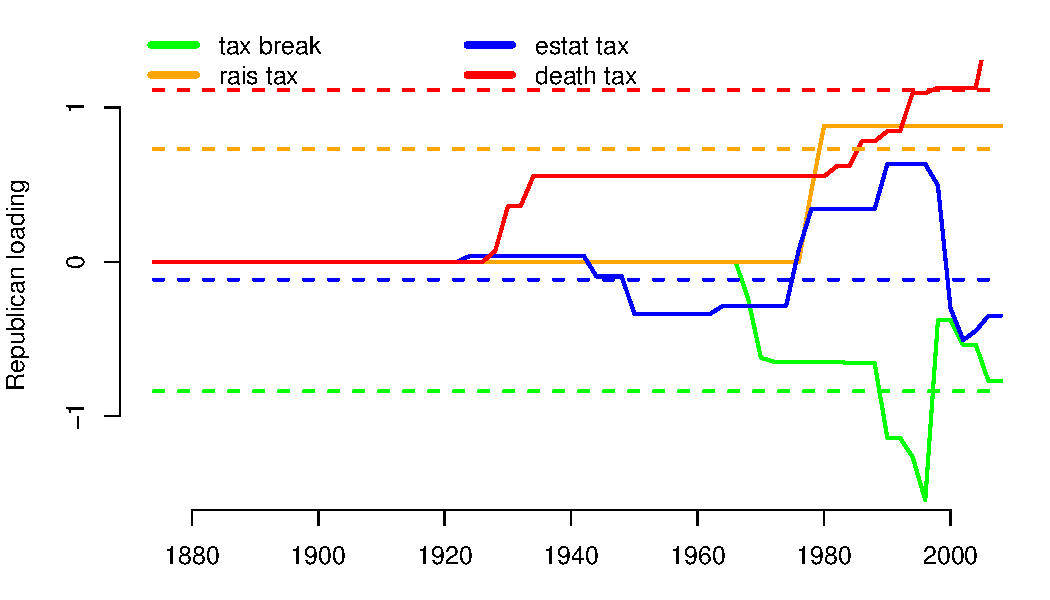
\includegraphics[width=\textwidth]{../graphs/loaded_tax}

\vskip .5cm
The resulting fit has $\varphi_{tj}$ changing as a step function in $t$.

\end{frame}


\begin{frame}{Dynamic Phrase-Party Loadings: Race}

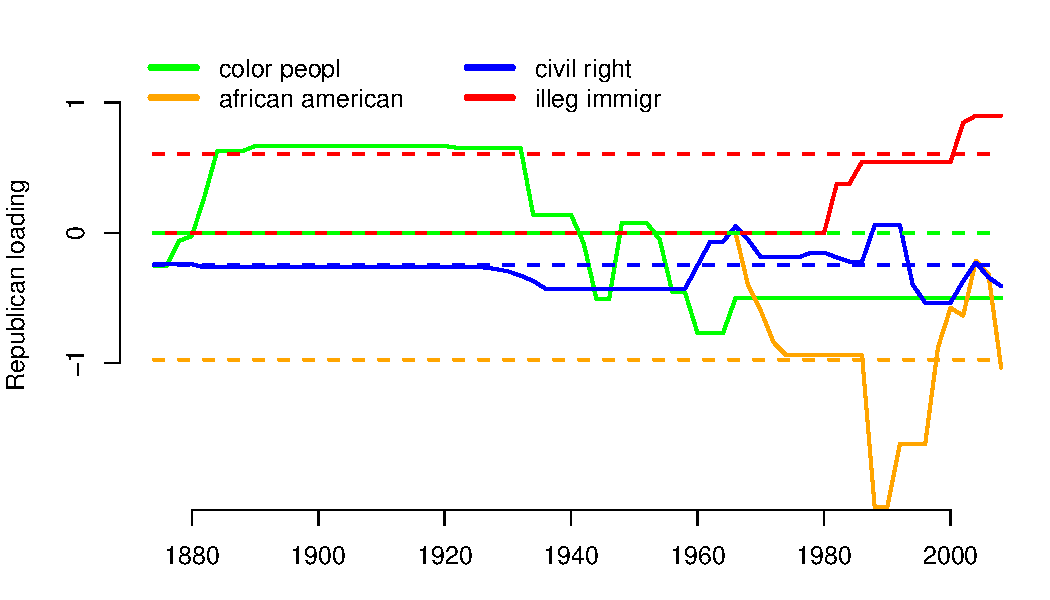
\includegraphics[width=\textwidth]{../graphs/loaded_race}

\vskip .5cm
For this example, partisanship is robust to fixing $\varphi_{tj} = \varphi_{j}$.
\end{frame}

\begin{frame}{Polarization Results: Baseline Specification}


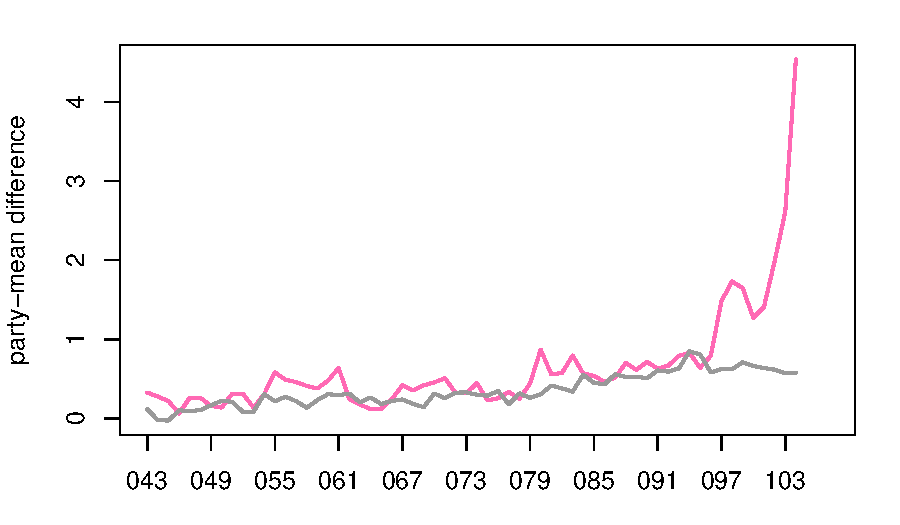
\includegraphics[width=\textwidth]{../graphs/bic-polars}

\vskip .5cm
We take $\bar z_{rt} = \frac{1}{n_{rt}} \sum_{i: r_i=r} z_{it}$ for
each party in each session, \\and the difference is our partisanship index.

\vskip .25cm
{\theme Partisanship of rhetoric has exploded since around 1980.}
\vskip -.25cm
\end{frame}

\begin{frame}{Nonparametric Bootstrap}


\includegraphics[width=\textwidth]{../graphs/boot-bic-polars}

\vskip .5cm
1980 is also when real partisanship becomes more than \\$2SE$ away from that for random permutations.

\end{frame}

\begin{frame}{Penalization is a necessary ingredient}


\includegraphics[width=\textwidth]{../graphs/noc-polars}


\vskip .5cm
These are the results corresponding to the end of each lasso path (most complex model)
\end{frame}

\begin{frame}{Robustness}


\includegraphics[width=\textwidth]{../graphs/bic-polars_all}

\vskip .5cm
With BIC penalty selection, the same shape holds under a variety of specifications.  {\color{black!50} But notice: the controls do make a  difference.}
\end{frame}

\begin{frame}{Another application: racial segregation on the internet}

ComScore browser histories on the websites used in Gentzkow \texttt{+} Shapiro (2011), making visit-counts a function of $r_{it}$ black/white.

\vskip .25cm
\includegraphics[width=\textwidth]{../graphs/Comscore-polars}

\vskip .25cm

Segregation online is high, but has been dropping since 2004.

\vskip -.25cm

\end{frame}

\begin{frame}{Conclusion}

We've written down a model for choices, \\and defined segregation in terms of that model.

\vskip .5cm
We can specify time dynamics and covariates inside this model.

\vskip .5cm
The same techniques that allow machine learners to avoid overfit in prediction can be used to recover representative model fits.

\vskip 1cm
\centering \huge \theme Thanks!

\end{frame}

\end{document}
























